\documentclass[portrait,a0paper]{baposter}

% Includes
\usepackage[utf8]{inputenc}
\usepackage[german]{babel}
\usepackage{graphicx}
\usepackage{amsmath}
\usepackage{amssymb}

% Colors
\definecolor{bggrey}{RGB}{230,230,230}
\definecolor{boxheader}{RGB}{81,173,113}
\definecolor{boxbg}{RGB}{181,181,181}

\begin{document}
\begin{poster}
%poster params
  {
  grid=false,
  bgColorOne=bggrey,
  background=plain,
  headerColorOne=boxheader,
  headershape=smallrounded,
  headerborder=none,
  headershade=plain,
  boxshade=plain,
  boxColorOne=boxbg,
  eyecatcher=false
  }
% Eye-catcher
  { } 
% Title
 {\bf\textsc{Robotersteuerung mit einer Kinect}\vspace{0.5em}}
% Authors
  {
  \textsc{Interdisciplinary Center for Scientific Computing}  \vspace*{0.5em} \\
  \small \textsc{Matthias.Hummel@stud.uni-heidelberg.de} \\
  \small \textsc{Manuel.Dewald@stud.uni-heidelberg.de}
  }
% Logo
  {% The makebox allows the title to flow into the logo, this is a hack because of the L shaped logo.
    
\includegraphics[width=100px]{imgs/IWRlogo1.png}
  }
  
%%%%%%%%%%%%%%%%%%%%%%%%%%%%%%%%%%%%%%%%%%%%%%%%%%%%%%%%%%%%%%%%%%%%%%%%%%%%%%
    \headerbox{Problem}
    {
    name=problem,
    column=0,
    row=0,
    textborder=none
    }
    {
Ziel des Praktikums ist die Steuerung eines Greifarms mithilfe einer Kinect.
Bestimmte Bewegungsmuster werden von der Kinect erkannt auf einen mechanischen Greifarm übertragen.
Hierzu soll eine Schnittstelle zwischen der Kinect-API und der Steuerung des Roboters implementiert werden.
Die Steuerung des Roboters soll hierbei möglichst Intuitiv mit den Armen durchführbar sein:
Der Benutzer stellt sich in den Steuerungsbereich, wird von der Kinect erkannt und kann anschließend mit wenig Übung den Roboterarm an die gewünschte Position bringen und Gegenstände greifen.
 }
%%%%%%%%%%%%%%%%%%%%%%%%%%%%%%%%%%%%%%%%%%%%%%%%%%%%%%%%%%%%%%%%%%%%%%%%%%%%%%

%%%%%%%%%%%%%%%%%%%%%%%%%%%%%%%%%%%%%%%%%%%%%%%%%%%%%%%%%%%%%%%%%%%%%%%%%%%%%%
    \headerbox{Vorgehen}
    {
    name=Vorgehen,
    column=0,
    below=problem,
    textborder=none
    }
    {
\textbf{Komponenten}

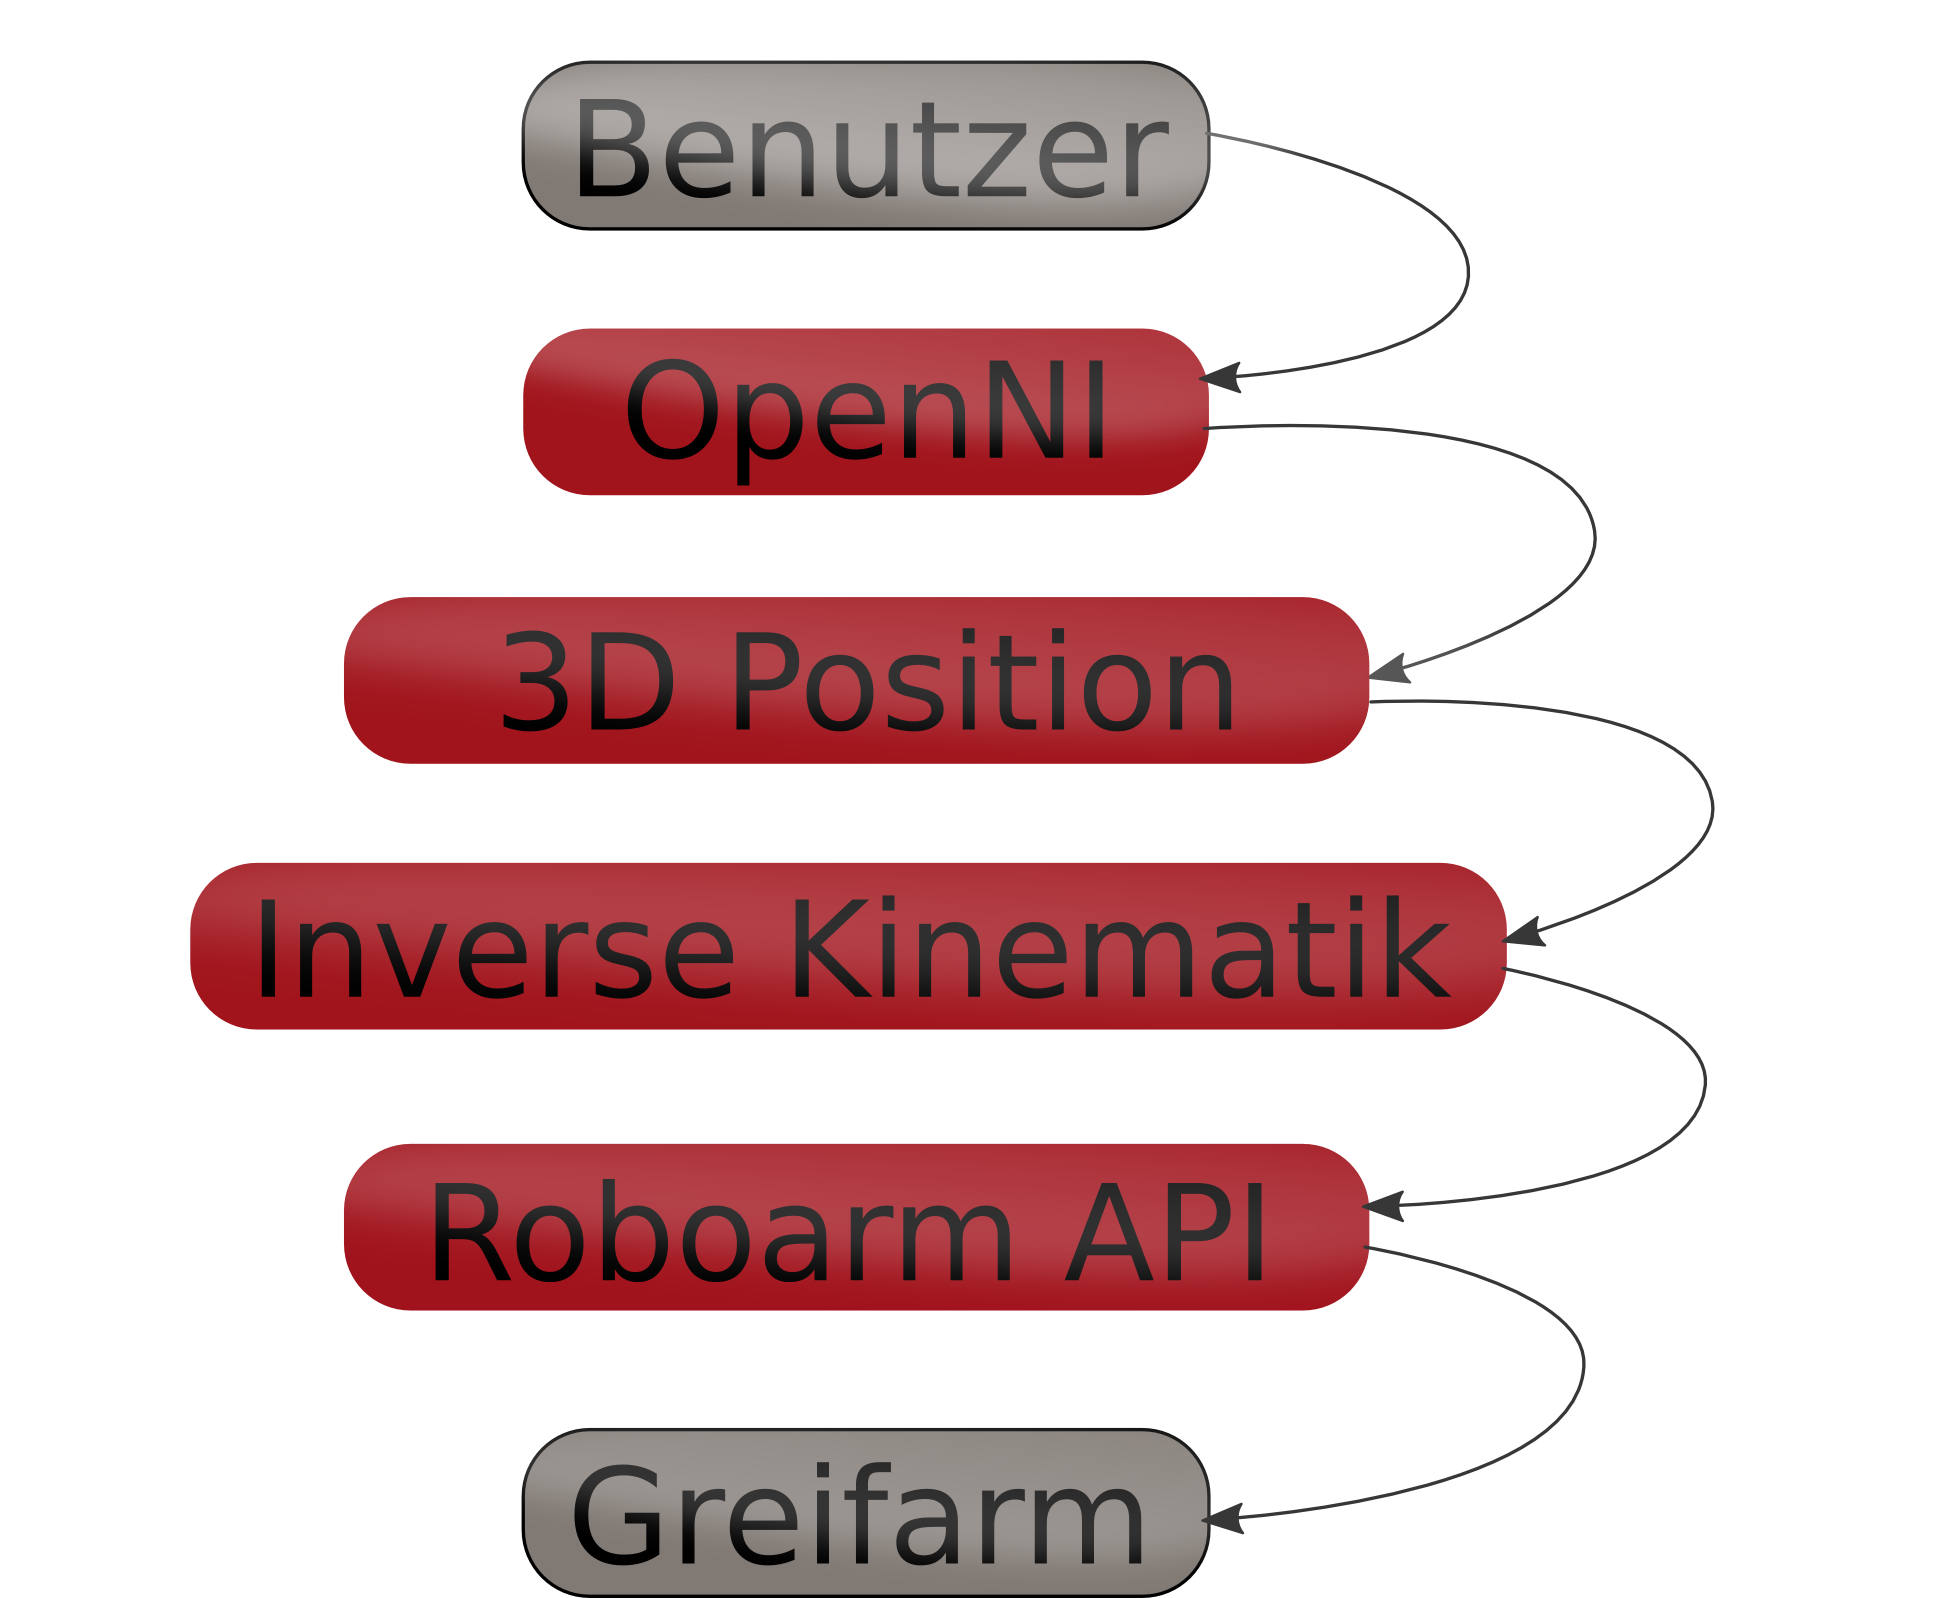
\includegraphics[width=\textwidth]{imgs/komponenten.png}

Die Microsoft Kinect trackt die Bewegungen des Benutzers welche dann über das OpenNI-Interface ausgelesen werden können. Dieser Output wird für die Inverse Kinematik verwendet um den Roboter entsprechend zu steuern.
 }
%%%%%%%%%%%%%%%%%%%%%%%%%%%%%%%%%%%%%%%%%%%%%%%%%%%%%%%%%%%%%%%%%%%%%%%%%%%%%%






%%%%%%%%%%%%%%%%%%%%%%%%%%%%%%%%%%%%%%%%%%%%%%%%%%%%%%%%%%%%%%%%%%%%%%%%%%%%%%
    \headerbox{Inverse Kinematik}
    {
    name=kinematik,
    column=1,
    span=2,
    row=0,
    textborder=none
    }
    {
        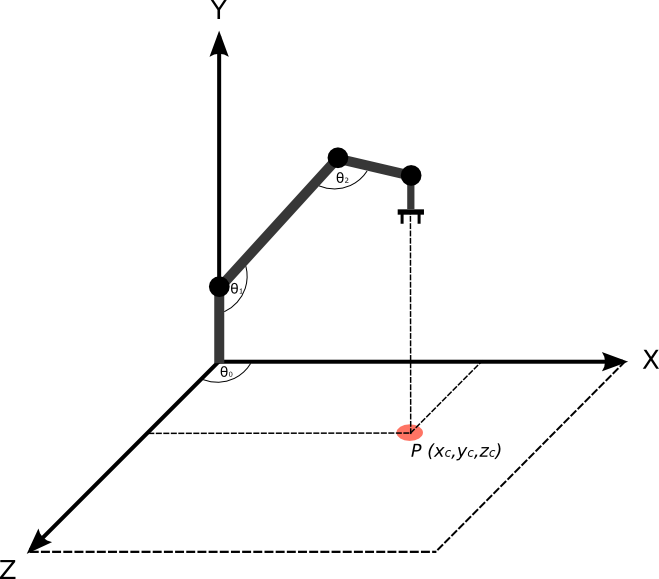
\includegraphics[width=\textwidth]{imgs/3d_robo.png}

 }
%%%%%%%%%%%%%%%%%%%%%%%%%%%%%%%%%%%%%%%%%%%%%%%%%%%%%%%%%%%%%%%%%%%%%%%%%%%%%%




\end{poster}
\end{document}